\documentclass[conference,10pt]{IEEEtran}
\usepackage[T1]{fontenc}
\usepackage[utf8]{inputenc}
\usepackage{amsmath,amssymb,amsthm}
\usepackage{booktabs}
\usepackage{tikz}
\usetikzlibrary{arrows.meta,positioning,shapes.misc,calc}
\usepackage{url}
\usepackage{xcolor}
\usepackage[hidelinks]{hyperref}

\newtheorem{proposition}{Proposition}
\newtheorem{definition}{Definition}
\newtheorem{corollary}{Corollary}
\newtheorem{lemma}{Lemma}

\newcommand{\PD}{P_{\mathrm{D}}}
\newcommand{\PDT}{P_{\mathrm{D}}(T)}
\newcommand{\PF}{P_{\mathrm{F}}}
\newcommand{\PO}{P_{\mathrm{O}}}
\newcommand{\Om}{\Omega}
\newcommand{\Bel}{\mathcal{B}}

\begin{document}

\title{Exactly-Once Effects for Regrouping Agent Tool Calls:\\
A Reduction, a Retention Hazard, and an Evidence Contract}

\author{\IEEEauthorblockN{Research-team working draft}
\IEEEauthorblockA{Version 0.3 --- 19 September 2026\\
Development results; not submitted; authorship confirmation pending}}

\maketitle

\begin{abstract}
A recovering language-model agent may re-express an authorized task with different tool calls. The runtime must decide which authorized effect occurrences remain available, not whether the new request text equals the old one. We study a restricted language of independent, explicitly authorized effect obligations executed against a durable sink. Three results follow. \emph{(i)~Reduction.} With a sink that atomically retains a per-key effect record for the whole recovery period, verified plan refinement reduces to stable obligation-key execution: a second implementation written from the v0.2 specification reproduces the v0.2 null result exactly across 186{,}674 exhaustively enumerated regrouping cases, 240 real SIGKILL/recovery trials and 24 three-worker races, and a reference that consults its own ledger dispatches the same set as the verifier by construction. \emph{(ii)~Retention hazard.} The two commercial idempotency contracts we examined are finite: Stripe prunes idempotency keys after at least 24~hours and treats a reused key as a new request; Amazon SQS FIFO deduplicates for 5~minutes. We model retention-bounded sinks $\PDT$, prove that same-key retry is safe against every history the controller cannot rule out exactly when its own hold timestamp is within the window less a stated end-to-end timing bound, and show that every same-key-retry policy---including the strong reference and the v0.2 verifier---duplicates in every lost-acknowledgement case once the window closes (149{,}217 of 186{,}674 enumerated cases, a seven-step model-checking witness, and 20/20 runtime duplicates for naive recovery versus 0/20 for the retention-aware controller). A lookup-then-fresh-key recovery without a fence---a hand-written handler, not the same-key retry a durable-execution engine prescribes---duplicates whenever the old request is still in flight (15/15 in-flight takeover trials, on every profile including the deduplicating one) and is correct whenever it has landed (0/15). Completion after the window then depends on an evidence contract: the retention-aware controller completed 10/10 lost-acknowledgement trials with a lookup endpoint and left 10/10 unresolved without one. \emph{(iii)~Evidence contract.} A ternary per-obligation projection is sufficient for the maximal safe fresh-dispatch set but not for reconciliation cost: retaining the processing class of a lost batch request changes the exact optimal expected number of per-item evidence calls from $n$ (independent entries) to $1$ (atomic) and to about $\log_2(n{+}1)$ (ordered stop-on-failure) when finality is provided per request, and to $4.5$ and $4.9$ of $8$ when every fresh dispatch must be preceded by a per-key fence and the policy minimises that total; a journal-driven recovery worker reproduces these counts on the runtime, and a misdeclared class produces false completion. A takeover study across three provider profiles shows where a fence, an evidence lookup and an explicit unresolved state each do work the others do not, and a resumed-predecessor study shows that a stale worker's receipt is evidence the controller can adopt without weakening its lease rule. No live LLM, commercial provider call, universal exactly-once guarantee or superiority over published systems is claimed.
\end{abstract}

\begin{IEEEkeywords}
agent systems, effect identity, crash recovery, idempotency, retention, authorization, partial observability
\end{IEEEkeywords}

\section{Introduction}

An agent instructed to send one deployment notification to each of two recipients can use one batch call, two single-recipient calls, or a different ordering. After a crash it may choose another representation. Asking whether the new request has the same text as the old one does not specify the recovery decision. The runtime must determine which authorized \emph{occurrences} are being attempted and what is known about their previous effects.

Three ambiguities must be separated. Identical payloads can belong to different approvals: a user may legitimately request the same notification again. One approval can produce different request representations without authorizing additional effects. And a request may have committed even though its result is absent from the checkpoint. Existing work addresses parts of this space: semantic rollback attacks and replay-or-fork recovery~\cite{acrfence}, durable authorization instances bound to canonical actions~\cite{caplease}, reservations under ambiguous provider outcomes~\cite{aidguard}, and task-level staged effects~\cite{cordon}. Durable-execution engines recommend that side-effecting steps be idempotent and restart each attempt from its initial state~\cite{temporal}; completion-record systems established durable request identity and atomic effect/result recording~\cite{rifl}.

The v0.2 study began from the hypothesis that preserving effect obligations across plan changes would add safety or completion beyond a strong durable-workflow reference, and found a null result. This version asks the follow-on question that the null result forces: \emph{under which provider contracts does stable-key execution stop being sufficient, and what must a controller then know?} Two answers turn out to be concrete and testable. First, the sink assumption behind the reduction---retention of the key/effect record throughout recovery---is not what commercial providers document. Stripe removes idempotency keys after they are at least 24~hours old and ``generate[s] a new request if a key is reused after the original is pruned''~\cite{stripe}; Amazon SQS FIFO deduplication lasts five minutes~\cite{sqsdedup}. A recovery that lands after the window is a retry into a sink that has forgotten the key. Second, when the sink no longer deduplicates, safe completion depends on outcome evidence, whose cost depends on what the controller's journal retained about the lost request.

Contributions:
\begin{enumerate}
\item A second implementation of the v0.2 kernel written from its specification by the same research process, reproducing every finite-domain count (Table~\ref{tab:d1}) and the process-crash and concurrency results. It is not an external replication. The reference is strengthened to consult its own ledger (R$^{+}$); Lemma~\ref{lem:tie} shows it dispatches the same set as the verifier, so the tie is structural rather than empirical.
\item A retention-bounded profile $\PDT$ with a condition for safe same-key retry that depends only on the controller's hold timestamp, the documented window and one end-to-end timing bound, necessary and sufficient when every attempt commits or dies within a lifetime shorter than the window, under an explicit adversarial timing model (Prop.~\ref{prop:retention}); the exhaustive enumeration in Table~\ref{tab:d1ttl}, whose counts are a corollary of the proposition and serve as an implementation check; a model-checking mutant with a seven-step witness; and a runtime study with a finite-TTL sink (Table~\ref{tab:i4}).
\item A takeover study in which a successor worker adopts a held occurrence while the crashed worker's request is still in flight, across $\PD$, $\PF$ and $\PO$ with three recovery policies: naive same-key retry (what a durable-execution engine does when the idempotency key is the activity identity), lookup-then-fresh-key without a fence (a hand-written handler), and profile-aware recovery (Table~\ref{tab:i3}). The middle policy is the realistic baseline; it fails exactly in the in-flight case. A resumed-predecessor study (Table~\ref{tab:i6}) shows that the ledger's lease-holder rule protects controller state but not the effect count, and that under $\PO$ the resumed worker carries the only finality evidence, which a ledger can adopt safely by distinguishing evidence binding from lease ownership.
\item A semantics-determined belief construction: recording the membership, order and processing class of a lost batch request determines the belief family for the atomic, prefix and independent classes; ternary projection discards it. Closed forms for the atomic and prefix classes are verified against an exact adaptive oracle to $n=10$, and the independent class to $n=8$, under two evidence-cost accountings; the per-key accounting minimises total fences rather than probe count (Table~\ref{tab:e4}); a recovery worker that rebuilds the belief family from a one-field-per-request journal reproduces the expected counts on the runtime and a misdeclared class yields false completion (Table~\ref{tab:i5}).
\item A measured negative finding about a common evaluation design: three-worker races resolved by controller reservation never reach the sink's deduplication path (0 of 96 sink calls), so they do not test the sink contract.
\end{enumerate}

The empirical scope remains explicit. Proposals are generated by combinatorial transformations, not by a live LLM. The provider performs synthetic database insertions. Finite enumerations are exhaustive only in the stated models; process schedules are sampled. Commercial contract facts are quoted from official documentation, not exercised against a live account.

\section{Background and Prior-Art Boundary}

\subsection{Durability and completion records}
Idempotent, uniquely identified messages are the classical answer to at-least-once delivery across trust boundaries~\cite{helland2007,helland2012}; sagas compensate rather than deduplicate and require the compensating action to be known~\cite{sagas}, which an agent's regrouped tool call typically is not. RIFL retains completion records with operations and addresses retry routing and record lifetime~\cite{rifl}. A persistent identifier alone is insufficient if the external mutation and the deduplication record can diverge, if retries reach non-coordinating sinks, or if the record is reclaimed. RIFL treats record lifetime as a system-controlled parameter; a commercial provider controls it unilaterally, which is the gap this version studies. Stream processors obtain exactly-once by making the sink participate in a transaction or a checkpoint epoch~\cite{flink,kafka}; an agent's effect provider offers neither, only a documented key contract. The HTTP \texttt{Idempotency-Key} draft standardizes the client-supplied key and the fingerprint check but explicitly leaves the retention period to the server~\cite{idempotencykey}.

CapLease binds authorization instances to canonical actions with durable budgets and transactional transitions; its Server Ledger reference prevents duplicate effects with an idempotent sink~\cite{caplease}. A result against regenerated keys therefore does not establish an advantage over that design; we do not execute CapLease.

\subsection{Agent-specific execution boundaries}
ACRFence analyzes regenerated calls and either reuses an old result or requires a fork~\cite{acrfence}. AID-Guard holds a reservation while an outcome is ambiguous and permits replacement only under terminal-result or no-effect/fencing conditions~\cite{aidguard}; our fence-then-fresh-key path follows that boundary. Cordon introduces task-level semantic transactions with result lineage and staged effects~\cite{cordon}; we do not claim all-or-nothing commit across obligations. Proof-carrying agent actions associate verifiable evidence with proposals~\cite{pca}; our checker is an exact contract check, not a certificate system. Tool-using agents in the ReAct and Toolformer families interleave reasoning with tool calls whose text is regenerated on every step~\cite{react,toolformer}; that regeneration is the source of the regrouping we study, and none of these systems addresses the identity of the effect across a crash.

\subsection{Durable execution and commercial idempotency}
At-most-once delivery with a bounded duplicate cache is classical: Birrell and Nelson's RPC~\cite{birrell}, Lampson's account of reliable messages~\cite{lampson}, and the synchronized-clock protocol of Liskov, Shrira and Wroclawski, which detects a duplicate after per-sender state has been discarded provided clocks stay within a known bound~\cite{liskov1991}. Leases~\cite{gray1989} and fencing tokens such as Chubby's sequencer~\cite{chubby} are the mechanisms behind our lease-holder rule and the $\PF$ fence. Workflow shims that make a non-idempotent service idempotent~\cite{ramalingam}, intent locks~\cite{olive}, and exactly-once serverless logs~\cite{beldi,boki} assume the shim can see the effect; an agent's tool provider generally cannot be wrapped that way. Durable Functions give a semantics for restarting an orchestration from its log~\cite{durablefunctions}. Temporal documents that an Activity ``be idempotent, so retries can be processed without duplicate side effects'' and that ``each attempt starts from the initial state''~\cite{temporal}. Deduplication is thus delegated to the effect provider, and a retry under the activity's own key is our \emph{naive} policy. Prop.~\ref{prop:retention} has the same shape as the synchronized-clock bound, with two differences that matter here: after expiry those protocols reject the duplicate, whereas Stripe accepts the pruned key as a new request, and $T$ is a vendor parameter the controller does not choose. Stripe saves the result of the first request under an idempotency key, compares incoming parameters to the original and errors on mismatch, and removes keys after at least 24~hours, after which a reused key produces a new request~\cite{stripe}. SQS FIFO deduplicates by \texttt{MessageDeduplicationId} within a 5-minute window and continues tracking the identifier after delivery~\cite{sqsdedup}. These are the only two documented windows we rely on; both are finite.

\subsection{Partial outcomes and evidence contracts}
SQS \texttt{SendMessageBatch} reports each entry individually and can mix successes and failures under HTTP~200~\cite{sqsbatch}; SES \texttt{SendBulkEmail} returns ``one object per intended recipient''~\cite{ses}. These are \emph{independent} per-entry semantics. Slack's \texttt{conversations.history} provides message evidence after the fact, but for some application classes it is rate limited to one request per minute with at most 15 objects~\cite{slackhistory}; and Slack's write method documents that on \texttt{fatal\_error} ``it's possible some aspect of the operation succeeded before the error was raised''~\cite{slackpost}, which is the opaque-outcome ambiguity in a vendor's own words. Planning with partial information and sensing is established~\cite{brafman,kaelbling}; our belief families are an application of that view with a set-valued, prior-uniform belief and unit-cost sensing, and our finite-state exploration follows the explicit-state model-checking tradition~\cite{spin} rather than proving the protocol in a theorem prover. Optimal decision trees are NP-complete in general~\cite{hyafil}, which is why the probe oracle is exponential and the closed forms are per class.

\section{Problem Model}

\subsection{Three identities}
An immutable approval contract is $C=(\iota,p,\alpha,\Om,s,v)$: intent-instance identifier, principal, authenticated approval event, finite set of obligation occurrence identifiers, approved effect specification per obligation, and schema version. An \emph{attempt} is a proposed or transmitted implementation of one or more obligations. An obligation identifies an occurrence, not a payload equivalence class; two identical notifications approved twice are two occurrences. The trusted approval layer creates $\iota$ and $\Om$; re-presenting the same $(p,\alpha)$ recovers the same contract.

The executable language supports exact tuples (kind, target, body) with kind \texttt{notify}, a singleton wrapper and a batch wrapper. Aliases, free-text inference, decomposition, cross-provider equivalence and state-dependent transformation are excluded. Obligations are independent.

\begin{proposition}[Content-only ambiguity]\label{prop:content}
A decision procedure observing only old and new payloads cannot always distinguish replay under one approval from an identical action under a new approval.
\end{proposition}
\begin{proof}
Completed $x$, lost receipt, repeated proposal yields observed input $(x,x)$; completed $x$ followed by a new approval for $x$ yields the same input. The required decisions differ. Approval provenance is the missing observation.
\end{proof}

\subsection{Failure and trust assumptions}
The proposer may reorder, regroup, omit, duplicate or alter proposed entries. The verifier rejects unauthorized entries before dispatching any prefix. Workers stop abruptly; concurrent workers may attempt the same obligations; a successor may adopt a held occurrence while the predecessor's request is still in flight. Conversation rollback never rolls back the contract, the control ledger or the provider ledger. Excluded: malicious host, corruption of both stores, lost disks, broken database atomicity, hostile clock manipulation beyond a bounded skew.

\subsection{Provider profiles, now with retention}
\begin{definition}[Profiles]
$\PDT$: atomic per-key effect/result recording with immutable key/payload binding, retained for at least $T$ after the first commit under the key; after $T$ the key may be reclaimed and a request under it may commit again. $\PD=\PDT$ with $T=\infty$. $\PF$: no key deduplication, but a fence operation that prevents any later delivery under a key and returns a trustworthy final outcome for it. $\PO$: neither; lookups are point-in-time only.
\end{definition}
Stripe's documented behaviour is $\PDT$ with $T\ge 24$~h and immutable parameter binding~\cite{stripe}; SQS FIFO is $\PDT$ with $T=5$~min~\cite{sqsdedup}. No profile is silently promoted to another; in particular a negative lookup alone never establishes $\PF$.

\section{Verified Refinement and Its Reduction}

\subsection{Plan checking and stable keys}
A plan contains an instance, schema and a sequence of wrapper groups. Verification checks the whole proposal: certified wrappers, legal arity, each slot approved and used at most once, and exact match of kind, target and body against the contract. Executable bytes are reconstructed from the contract. Partial plans are accepted; completed occurrences in a recovered plan are residualized and return cached completion.

The effect key is $K(\iota,\omega)=H(\texttt{obligation-key-v1},\iota,\omega)$, independent of grouping and attempt identity. Each occurrence has durable state $\mathit{ready}\to\mathit{held}\to\mathit{done}$; this version adds an $\mathit{unresolved}$ state, quiescent for the controller's own actions, for a held occurrence that can no longer be retried safely and for which the holder has no finality evidence. A control transaction reserves the occurrence (with a lease and, for $\PDT$, a retention deadline $h(\omega)+T$, where $h(\omega)$ is the controller time of this reservation) before transport.

\begin{figure}[t]
\centering
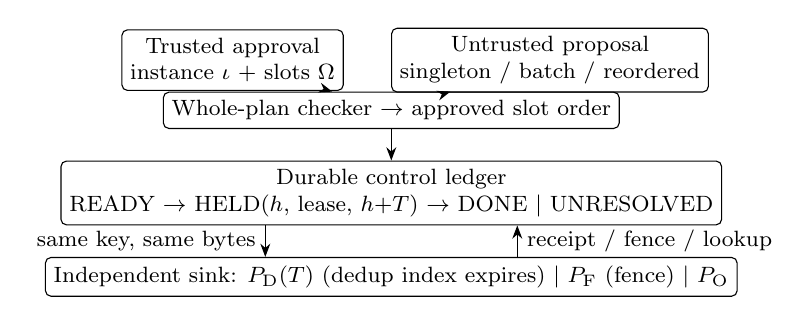
\begin{tikzpicture}[node distance=4mm and 6mm, every node/.style={font=\footnotesize}, box/.style={draw, rounded corners=2pt, align=center, inner sep=3pt, minimum width=2.4cm}]
\node[box] (approve) {Trusted approval\\instance $\iota$ + slots $\Om$};
\node[box, right=of approve] (plan) {Untrusted proposal\\singleton / batch / reordered};
\node[box, below=of $(approve)!0.5!(plan)$] (check) {Whole-plan checker $\to$ approved slot order};
\node[box, below=of check] (ledger) {Durable control ledger\\READY $\to$ HELD($h$, lease, $h{+}T$) $\to$ DONE $\mid$ UNRESOLVED};
\node[box, below=of ledger, minimum width=7cm] (sink) {Independent sink: $\PDT$ (dedup index expires) $\mid$ $\PF$ (fence) $\mid$ $\PO$};
\draw[-{Stealth}] (approve) -- (check);
\draw[-{Stealth}] (plan) -- (check);
\draw[-{Stealth}] (check) -- (ledger);
\draw[-{Stealth}] ([xshift=-1.6cm]ledger.south) -- node[left]{same key, same bytes} ([xshift=-1.6cm]sink.north);
\draw[-{Stealth}] ([xshift=1.6cm]sink.north) -- node[right]{receipt / fence / lookup} ([xshift=1.6cm]ledger.south);
\end{tikzpicture}
\caption{Implemented boundary. The sink effect is a synthetic database insertion. Recovery of a HELD occurrence consults $h(\omega)$, $T$ and the profile before choosing same-key retry, fence, evidence lookup or UNRESOLVED.}
\label{fig:boundary}
\end{figure}

\begin{proposition}[Stable-key reduction]\label{prop:reduction}
Assume immutable contracts, complete plan checking, mediated effect paths, an injective persistent key map, and $\PDT$ with every attempt under a key, the original included, committing before $h(\omega)+T$. Then any accepted sequence of regrouped plans and retries has at most one committed effect per approved occurrence and no effect outside the contract.
\end{proposition}
\begin{proof}
Every dispatched effect derives from an approved occurrence and its stored specification. All attempts for that occurrence use the same key. While the dedup record is retained, atomic key/effect recording allows at most one effect per key and rejects payload substitution. The retention hypothesis guarantees retention at every retry. Distinct occurrences are not collapsed by key identity. Induction over sink operations preserves the invariant.
\end{proof}

\begin{lemma}[Structural tie]\label{lem:tie}
Let $R^{+}$ validate the whole action list before dispatching any of it, then perform canonical-action matching per occurrence, skip occurrences recorded \emph{done} in the ledger and dispatch the rest under $K(\iota,\omega)$; let $V$ check the whole plan, residualize against the same \emph{done} set and dispatch the rest under the same keys. On any accepted destination plan both dispatch exactly the set of approved occurrences not recorded done, in the destination order, with identical bytes; hence identical sink calls and effect vectors.
\end{lemma}
\begin{proof}
Both filters compute ``approved and not done'' per occurrence. Because $R^{+}$ validates the whole list first, a rejected plan dispatches nothing in either policy; the checkers differ only on those rejected plans.
\end{proof}
The v0.2 reference $R$ resent every occurrence and let the sink deduplicate, so residualization saved calls without changing effects. In this artifact the abstract $R^{+}$ and $V$ share one code path and the runtime policy labeled $R$ in the process studies is this ledger-consulting $R^{+}$, not the resend-everything reference, so the equal counts in Table~\ref{tab:d1} check the implementation rather than test a hypothesis. Verified refinement adds no exactly-once guarantee under the retention hypothesis; the lemma is the null hypothesis for every comparison below.

\section{Finite Retention}

\subsection{The hazard}
The hypothesis ``every retry completes before $h(\omega)+T$'' is the load-bearing assumption of Prop.~\ref{prop:reduction}, and it is a property of the recovery \emph{schedule}, not of the code. A worker crash followed by an outage longer than $T$---or a checkpoint restored days later---violates it. The controller then holds an occurrence in state \emph{held} whose effect may or may not have committed; the sink has forgotten the key; and a same-key retry is indistinguishable, at the sink, from a first request.

\begin{proposition}[Retention-bounded same-key retry]\label{prop:retention}
Let the controller record $h(\omega)$ durably before transport and issue a same-key retry at controller time $t\ge h(\omega)$. Let $c$ be the earliest sink time at which the original attempt could commit and $a$ the sink time at which the retry arrives, and let the \emph{end-to-end timing error} $\varepsilon=(a-c)-(t-h(\omega))$ satisfy $|\varepsilon|\le\Delta$ in every admissible history. Let the attempt \emph{lifetime} be $L$: the original either commits at a sink time $c'$ with $c\le c'\le c+L$, or never commits. The adversary may choose any such history. On a $\PDT$ sink with $L+\Delta<T$, the retry is duplicate-free in every admissible history if and only if $t-h(\omega)<T-\Delta$. If $L+\Delta\ge T$, no such $t$ exists.
\end{proposition}
\begin{proof}
(If) Assume $L+\Delta<T$ and $t-h<T-\Delta$. If the original has committed at $c'$ before the retry arrives, its record lasts until at least $c'+T\ge c+T$, while $a\le c+(t-h)+\Delta<c+T$, so the retry is deduplicated. If it has not, the retry is the first commit and its record lasts until at least $a+T$. The original can still commit only at some $c'\le c+L$. Since $a\ge c+(t-h)-\Delta\ge c-\Delta$ and $L<T-\Delta$, one has $c'\le c+L<c+T-\Delta\le a+T$, so that late commit meets the retry's record and is deduplicated too. (Only if) If $t-h\ge T-\Delta$, the adversary commits the original at exactly $c$, which any $L\ge 0$ allows, and chooses $\varepsilon=\Delta$; then $a\ge c+T$, the record may have been reclaimed, and the retry commits a second effect. If instead $L+\Delta\ge T$, the adversary lets the retry commit first and lands the original at $c+L$ after the retry's record expires, for every $t$; that is the in-flight duplicate of Table~\ref{tab:i3} moved onto a short window.
\end{proof}
For clocks with a constant offset, $\Delta$ is the maximum sink-side delivery delay of the retry relative to the original; if the offset can change between hold and retry, $\Delta$ additionally includes twice the skew bound. $L$ is a provider fact too: an attempt the provider can still execute after the retention window is not covered by same-key retry at any $t$. The documented windows we use, at least 24~hours and 5~minutes, sit well above a request's network lifetime, which is why the regime $L+\Delta<T$ is the one that applies to them; we did not measure $L$. The studies below use $\Delta=0$ on one machine, so they exercise the window, not the margin.

The decision uses only the controller's own ledger and two contract parameters, $T$ and $\Delta$. No sink query can substitute for it: a negative lookup after reclamation is consistent with both histories.

\begin{corollary}[Profile downgrade]\label{cor:downgrade}
After $h(\omega)+T-\Delta$, a key on a $\PDT$ sink is no longer deduplicated. For that key the sink is then at best $\PF$, if it exposes a fence or another finality operation, and $\PO$ otherwise.
\end{corollary}
\begin{definition}[Retention-aware recovery]\label{def:aware}
Inside the bound of Prop.~\ref{prop:retention} the controller retries the same key. After it, positive point-in-time evidence confirms; a fence permits a fresh key; a negative point-in-time lookup establishes nothing, so absent a fence the occurrence becomes \emph{unresolved}.
\end{definition}

Where the objects a request created remain retrievable after the key is pruned---as Stripe's list endpoints permit for created objects, a capability we did not exercise here---the sink degrades to a lookup-capable profile; SQS offers no message lookup by deduplication identifier, so it degrades to $\PO$. The controller must therefore carry $T$ and the evidence capability as explicit provider-contract fields.

\subsection{Ambiguous replacement}
A fresh key is different from a same-key retry. Certifying absence from a negative lookup and then dispatching a fresh key permits two distinct keys to commit one obligation if the old request can still arrive. Safe replacement in $\PF$ needs an operation that certifies no old effect and prevents old delivery~\cite{aidguard}; Section~\ref{sec:results-i3} exercises this with a real in-flight request.

\section{Outcome Knowledge Beyond Independent States}\label{sec:belief}

\subsection{Safe fresh-dispatch frontier}
Under $\PF$, let a nonempty belief family $\Bel\subseteq 2^{\Om}$ contain every finalized committed set consistent with sound evidence. Define $P(\Bel)=\bigcup\Bel$, $D(\Bel)=\bigcap\Bel$, $F(\Bel)=\Om\setminus P(\Bel)$ and $U(\Bel)=P(\Bel)\setminus D(\Bel)$.
\begin{proposition}[Maximal safe fresh dispatch]\label{prop:frontier}
A once-only fresh dispatch set $S$ is duplicate-free in every world of $\Bel$ iff $S\subseteq F(\Bel)$.
\end{proposition}
\begin{proposition}[No-observation completion boundary]\label{prop:singleton}
A single fixed fresh dispatch set both avoids duplicates and completes every obligation in every world of $\Bel$ iff $|\Bel|=1$.
\end{proposition}
\begin{proof}[Proof of Prop.~\ref{prop:frontier}]
$S$ is duplicate-free in world $w$ iff $S\cap w=\emptyset$; for all $w\in\Bel$ iff $S\cap\bigcup\Bel=\emptyset$ iff $S\subseteq F(\Bel)$.
\end{proof}
\begin{proof}[Proof of Prop.~\ref{prop:singleton}]
Completion in $w$ requires $S\supseteq\Om\setminus w$ and duplicate-freedom requires $S\cap w=\emptyset$, so $S=\Om\setminus w$; one $S$ serves two worlds only if they are equal.
\end{proof}
Both statements are definitional once the belief family is fixed; E1 evaluates them exhaustively as a check of the artifact's code, not as evidence. Both depend on fresh mutation, no new observation and old-dispatch finality; a $\PD$ sink within its window can replay retained keys without identifying the completed set.

\subsection{Safety sufficiency is not query sufficiency}
The ternary projection (done on $D$, absent on $F$, unknown on $U$) determines $F$ exactly, so correlations never enlarge the immediate safe frontier. They change the cost of learning more. The v0.2 witness $\Bel_1=\{\{a\},\{b\}\}$ versus $\Bel_2=2^{\{a,b\}}$ has identical projections and optimal probe costs one and two.

\subsection{Semantics-determined belief families}
The source of correlation in practice is not exotic: it is the processing semantics of the request whose response was lost. Let a request carry ordered members $M=(\omega_1,\dots,\omega_n)$ and let the journal record $M$, its order and the provider's documented processing class.
\begin{definition}[Classes]
\emph{independent}: any subset may have committed ($\Bel=2^{M}$; per-entry outcomes as in SQS batch and SES bulk~\cite{sqsbatch,ses}). \emph{atomic}: all or nothing ($\Bel=\{\emptyset,M\}$; a single-object request such as one Stripe charge~\cite{stripe}). \emph{prefix}: ordered processing that stops at the first failure ($\Bel=\{\{\omega_1..\omega_k\}:0\le k\le n\}$; the sequential worker of this artifact executing a batch wrapper is one instance). \emph{exact-$k$}: a trustworthy aggregate reports $k$ successes ($\Bel=\binom{M}{k}$).
\end{definition}
\begin{proposition}[Journal sufficiency and probe costs]\label{prop:classes}
For the independent, atomic and prefix classes, recording $(M,\text{order},\text{class})$ before transport determines $\Bel$; the exact-$k$ family additionally requires one post-hoc aggregate evidence call to learn $k$. Every class projects to all-unknown on $M$, so a ternary journal believes $2^{M}$ and needs $n=|M|$ unit probes. Under a uniform prior over worlds and unit-cost per-item probes, the exact optimal adaptive expected cost is $n$ (independent), $1$ (atomic), $\lceil\log_2 N\rceil-\frac{2^{\lceil\log_2 N\rceil}-N}{N}$ with $N=n{+}1$ (prefix), and $1+n-\frac{n-k}{k+1}-\frac{k}{n-k+1}$ (exact-$k$, including the aggregate call).
\end{proposition}
\begin{proof}
Determination is by construction of the families. Independent: a probe reveals one independent bit, so $n$ probes are necessary and sufficient. Atomic: any single probe identifies the world. Prefix: worlds are the $N$ prefixes ordered by length; probing $\omega_i$ splits the current candidate interval of lengths into the two contiguous sub-intervals $\{\ge i\}$ and $\{<i\}$, and conversely every split of a contiguous interval at a boundary is realized by probing the boundary item, so adaptive policies are exactly the binary decision trees over $N$ ordered, equally likely leaves. Expected depth is minimized by the complete tree, whose leaves lie at depths $\lfloor\log_2 N\rfloor$ and $\lceil\log_2 N\rceil$ with $2^{\lceil\log_2 N\rceil}-N$ at the shallower depth. Exact-$k$: the v0.2 gap-symmetry argument with the count-aware stopping rule, plus the aggregate call. Under per-key finality the objective is no longer the probe count. A probe of an absent member is the fence that member needs before a fresh dispatch, so it adds no further call, and a probe of a committed member is overhead. The optimum is then $(n+1)/2$ for the atomic class (any single probe), $n/2+n/(n+1)$ for the prefix class (scan from the end of the request and stop at the first committed member) and $n$ for the independent class. The probe-minimising prefix policy is the wrong policy for this objective: at $n=8$ it costs $5.8$ calls where the scan costs $4.9$. A dynamic program over the belief family matches these closed forms for every $n\le 10$ (independent through $n\le 8$). The worst case under per-key finality is $n$ for every class, the world in which nothing committed.
\end{proof}
Two accountings of evidence cost are relevant. \emph{Per-request finality}: the provider guarantees (by acknowledgement, SLA or a request-level finalize operation that returns no per-item outcome) that the lost request is finished; probes are then the only cost and fresh dispatch of certainly-absent items needs no further call. \emph{Per-key finality}: the only final evidence is a per-key fence; every absent item must be fenced before its fresh dispatch, a probe counts as that item's fence, and the cost is the quantity minimised in the proof. Table~\ref{tab:e4} reports both. The class is a property the controller already reads from provider documentation to choose a profile; retaining it per request costs one field. Like $T$, it is trusted contract data: a misdeclared class makes the controller infer completion that did not happen.

\section{Implementation and Reproducibility}

The v0.3 artifact is a fresh implementation written from the v0.2 manuscript rather than from its source tree, in Python standard library plus SQLite. Controller and provider run in different processes with different database files, WAL mode and \texttt{synchronous=FULL}. The controller stores immutable contracts, key/payload bindings, occurrence states with lease and retention deadline, receipts and events; insertion is transactional and $(p,\alpha)$ is unique. The provider inserts one row per effect atomically; a $\PDT$ dedup row carries an expiry; a $\PF$ fence table is consulted inside the effect transaction so an in-flight request that arrives after the fence is rejected; every \texttt{/execute} call is logged with its outcome so attempts are distinguishable from effects. An evidence endpoint searches the retained effect table, modelling providers whose history outlives their idempotency window; it can be disabled.

Two policies share transport and persistence. $R$ performs flat canonical-action matching and consults the ledger per occurrence; $V$ checks typed wrapper membership on the whole plan and residualizes. Three recovery modes exist for a held occurrence: \emph{naive} (same-key retry regardless of profile or retention); \emph{lookup-then-fresh} (query the evidence endpoint and, on a negative answer, dispatch under a fresh key without fencing, which is a hand-written handler; a durable-execution retry keyed by activity identity is the naive policy); and \emph{aware} (Def.~\ref{def:aware}). Ledger writes that confirm or abandon an occurrence are accepted only from the current lease holder, so a predecessor that resumes after a takeover cannot overwrite the successor's state. Two exceptions are studied in I6. A receipt whose key and payload hash bind to an occurrence already \emph{unresolved} may be adopted (\emph{adopt}) or refused (\emph{reject}). A binding-matched receipt that arrives while the successor still holds the occurrence is stored and adopted if the holder later gives up, and dropped if the holder rekeys, because the key no longer matches. Three invariants carry this: \texttt{reserve} refuses \emph{unresolved}, so the controller never fresh-dispatches from that state; \texttt{rekey} requires the holder; adoption requires the current binding. The worker's fault action is either SIGKILL or SIGSTOP; a stopped worker is resumed by the orchestrator with SIGCONT. For the evidence study the worker can send a wrapper group as one multi-entry request; the provider processes entries by a declared class (independent, atomic, prefix) with a per-entry failure hook, and the controller journals membership, order and class before transport. A recovering worker with a \emph{ternary} journal probes every held member; with a \emph{structured} journal it rebuilds the belief family of Section~\ref{sec:belief} and probes by the exact oracle. The probe is either a point-in-time lookup (per-request finality supplied by the study's timing) or a per-key fence (per-key finality), and in the latter accounting every absent member is fenced before its fresh dispatch. The successor may also be started with a journal class that contradicts the provider's actual processing, to measure the trusted-contract failure mode. Fault points terminate the process with a real SIGKILL after the first reservation, after the first effect before confirmation, after the first confirmation, after the third effect, or during the first transport (a timer kills the process 150~ms after the request is sent while the provider delays commit).

The artifact contains 37 kernel unit tests, all experiment drivers, raw per-trial records (635 process trials with return codes, crash markers, successor summaries and provider-side counts), exhaustive enumerations and model-checking witnesses. \texttt{run\_all.py} regenerates every number in this paper in about fifteen minutes on one core. Manifests are local provenance, not external timestamping.

\section{Study Design}

\textbf{D1 and D1-TTL.} For $n=1..4$, enumerate all $n!\,2^{n-1}$ ordered groupings as source and destination and every committed prefix of the source order: $\sum_{n=1}^{4}(n!\,2^{n-1})^2(n{+}1)=186{,}674$ cases. Policies: $G$ (group-scoped key), $R$, $R^{+}$, $V$, $V_r$ (retention-aware, no evidence), $V_r{+}E$ (retention-aware with lookup). Six variants cross the state of the last committed occurrence at the crash---durably confirmed, committed with lost acknowledgement, or reserved without effect---with whether the dedup index was reclaimed before recovery.

\textbf{M1.} One obligation, two key generations, two senders per generation, one crash, plus a retention-expiry transition that fires only while no request is in flight. Breadth-first search exhausts the safe configuration; each mutant stops at its shortest violating trace. State counts are specific to this encoding and not comparable to v0.2's.

\textbf{I1, I2.} As in v0.2: 2 policies $\times$ 6 source/destination grouping pairs $\times$ 4 fault points (after the first reservation, after the first effect, after the first confirmation, and after the third effect) $\times$ 5 repetitions $=240$ SIGKILL/recovery trials on $\PD$. The during-transport fault is used by I3, I5 and I6 rather than by I1. I2 is 12 three-worker races per policy. The runtime policy labeled $R$ consults the ledger, so it is $R^{+}$ of Table~\ref{tab:d1}.

\textbf{I3.} Source plan one batch of four; the worker is killed 150~ms into its first transport while the provider delays commit by 1000~ms (\emph{early}) or 200~ms (\emph{late}). A different worker adopts the held occurrence after lease expiry at 0.5~s or 0.9~s. $3$ profiles $\times$ $2$ variants $\times$ $3$ recovery modes $\times$ 5 repetitions $=90$ trials. The evidence endpoint is enabled for every profile so that lookup-then-fresh has the information it would have in practice.

\textbf{I4.} $\PDT$ with $T=0.5$~s. The worker is killed after the first effect (lost acknowledgement) or after the first reservation (no effect); the successor starts $0.8$~s later. $2$ evidence settings $\times$ $2$ faults $\times$ $2$ recovery modes $\times$ $2$ policies $\times$ 5 $=80$ trials.

\textbf{I6.} As I3, but the predecessor is SIGSTOPped after its first reservation or 150~ms into its first transport (provider commit delay 1000~ms), the successor recovers with the aware policy at 0.5~s, and the predecessor is resumed at 1.6~s and runs to completion. $3$ profiles $\times$ $2$ stop points $\times$ $2$ late-evidence rules $\times$ 5 $=60$ trials.

\textbf{I5.} One batch request over $n$ members is sent and the worker is killed before it can read the response; the provider fails the entries designated by the world. Every world of each class is run once: independent $n{=}4$ (16 worlds), atomic $n{=}4,8$ (2 each), prefix $n{=}4,8$ (5 and 9). The successor starts after the provider finished (finality by construction), reconciles from a ternary or a structured journal, confirms committed members and fresh-dispatches absent ones under new keys on $\PF$. There are 34 worlds (16 independent, 2+2 atomic, 5+9 prefix). Each is run under both journals and both accountings (136 trials); 5 further prefix worlds are run with the journal misdeclaring the class as atomic. $141$ trials. Under per-key finality the structured journal uses the fence-minimising policy of Prop.~\ref{prop:classes}, which is not the probe-minimising policy.

\textbf{E1--E4.} E1 enumerates all $65{,}535$ belief families on four occurrences against all 16 dispatch sets. E2 is the correlation witness. E3 compares the exact-$k$ closed form with an exact dynamic-programming oracle for all $0<k<n\le 10$ (2{,}026 worlds; v0.2 stopped the oracle at $n=8$). E4 computes ternary and structured optimal probe costs for the independent, atomic and prefix classes.

The success oracle for every process trial requires the crashed worker to exit with $-9$, the successor with $0$, and reads the provider's effect table independently of controller state.

\section{Results}

\subsection{The reduction holds and the strengthened reference ties}
\begin{table}[t]
\centering\footnotesize
\caption{D1: exhaustive regrouping on $\PD$ with unbounded retention. Duplicates are case counts, not agent failure rates. $R^{+}$ and $V$ have identical effect vectors in every case and identical call counts.}
\label{tab:d1}
\begin{tabular}{@{}rrrrrrr@{}}
\toprule
$n$ & Plans & Cases & $G$ dup & $R$ dup & $R^{+}$ dup & $V$ dup\\
\midrule
1 & 1 & 2 & 0 & 0 & 0 & 0\\
2 & 4 & 48 & 16 & 0 & 0 & 0\\
3 & 24 & 2{,}304 & 1{,}308 & 0 & 0 & 0\\
4 & 192 & 184{,}320 & 129{,}024 & 0 & 0 & 0\\
\midrule
Total & & 186{,}674 & 130{,}348 & 0 & 0 & 0\\
Sink calls & & & 744{,}290 & 744{,}290 & 372{,}145 & 372{,}145\\
\bottomrule
\end{tabular}
\end{table}
Table~\ref{tab:d1} reproduces the v0.2 counts exactly (16 / 1{,}308 / 129{,}024 group-key duplicates) from an independent implementation. $R^{+}$ and $V$ agree on every effect vector and make the same 372{,}145 calls; $R$ makes twice as many because it resends completed occurrences and lets the sink deduplicate. In I1 all 240 trials pass for both policies; the provider logs 1{,}080 execute calls for 960 effects, and the 120 excess calls are exactly the lost-acknowledgement retries (60 trials each at the after-first-effect and after-third-effect fault points) answered with a cached receipt. In I2 all 24 races pass; the provider logs 96 calls, all committed, none deduplicated---controller reservation resolves every race before the sink is reached. Median successor wall time is 0.101~s ($R$) and 0.102~s ($V$) including interpreter start; it is descriptive only.

\subsection{After the window, every same-key policy duplicates}
\begin{table}[t]
\centering\footnotesize
\caption{D1-TTL: the same 186{,}674 cases when the dedup index is reclaimed between crash and recovery. \emph{dup}: cases with a duplicated occurrence; \emph{unres}: cases the controller leaves unresolved; \emph{inc}: cases where an approved occurrence never happened.}
\label{tab:d1ttl}
\setlength{\tabcolsep}{3.5pt}
\begin{tabular}{@{}llrrrr@{}}
\toprule
Last occ.\ at crash & Policy & dup & unres & inc & calls\\
\midrule
confirmed & $R$ & 149{,}217 & 0 & 0 & 744{,}290\\
 & $R^{+}$, $V$ & 0 & 0 & 0 & 372{,}145\\
 & $V_r$, $V_r{+}E$ & 0 & 0 & 0 & 372{,}145\\
\midrule
lost ack & $R$ & 149{,}217 & 0 & 0 & 744{,}290\\
 & $R^{+}$, $V$ & 149{,}217 & 0 & 0 & 521{,}362\\
 & $V_r$ & 0 & 149{,}217 & 0 & 372{,}145\\
 & $V_r{+}E$ & 0 & 0 & 0 & 521{,}362\\
\midrule
reserved, no effect & $R$ & 111{,}760 & 0 & 0 & 744{,}290\\
 & $R^{+}$, $V$ & 0 & 0 & 0 & 521{,}362\\
 & $V_r$ & 0 & 149{,}217 & 149{,}217 & 372{,}145\\
 & $V_r{+}E$ & 0 & 149{,}217 & 149{,}217 & 521{,}362\\
\bottomrule
\end{tabular}
\end{table}
Table~\ref{tab:d1ttl} is the finite-domain form of Prop.~\ref{prop:retention}. With reclaimed retention and a lost acknowledgement, $R$, $R^{+}$ and $V$ all duplicate in every one of the 149{,}217 cases with a nonempty committed prefix. The verifier's plan-level residualization protects only occurrences the controller already recorded as done. The retention-aware policy is safe in every variant; without evidence it pays with 149{,}217 unresolved cases, which are false alarms under lost acknowledgement and real gaps when nothing had committed. With a lookup it completes every lost-acknowledgement case at one evidence call per lapsed occurrence, but in the reserved-without-effect variant its negative lookup is not finality evidence, so it stops at \emph{unresolved} exactly as $V_r$ does and has paid one more call to learn nothing it could act on; this is the abstract counterpart of the ``after reservation, aware, lookup'' row of Table~\ref{tab:i4}. Without retention expiry, all six policies except $G$ are safe and complete in all three crash-state variants. We stress that these counts are a consequence of the proposition applied to each case, not independent evidence for it: the enumeration checks that the implementation of $V_r$ behaves as specified on every regrouping, which is its purpose.

\subsection{Model checking}
\begin{table}[t]
\centering\footnotesize
\caption{M1 bounded reachability. Only safe rows exhaust their graph; mutants stop at the shortest witness.}
\label{tab:m1}
\begin{tabular}{@{}llrrl@{}}
\toprule
Model & Configuration & States & Edges & Witness\\
\midrule
v0.2 & safe & 1{,}180 & 3{,}467 & none (exhausted)\\
 & absence without fence & 445 & 1{,}036 & 9 (duplicate)\\
 & fresh-key retry & 395 & 939 & 7 (duplicate)\\
 & missing as success & 11 & 11 & 2 (false success)\\
 & no sink dedup & 65 & 126 & 6 (duplicate)\\
\midrule
+retention & safe & 1{,}396 & 4{,}043 & none (exhausted)\\
 & retry after expiry & 121 & 249 & 7 (duplicate)\\
 & safe, no fence capability & 76 & 158 & none (exhausted)\\
\bottomrule
\end{tabular}
\end{table}
The retention mutant's witness is: hold, send, commit, crash, retention expires, resend same key, commit. The safe configuration with the retention transition still exhausts without violation because its send rule refuses any key that may have been dispatched before expiry; recovery proceeds through fence, lookup and certificate instead. The last row removes the fence transition to model a $\PDT$ sink that offers no fence: the safe controller still exhausts without a duplicate or false success, in a much smaller graph, because after expiry its only remaining move for a possibly-dispatched key is to stop. M1 checks safety only; it does not check liveness, and that row is precisely the configuration in which the controller can be safe by never completing.

\subsection{Takeover with an in-flight request}\label{sec:results-i3}
\begin{table}[t]
\centering\footnotesize
\caption{I3: a successor adopts a held occurrence while the crashed worker's request is still in flight (\emph{early}) or after it committed (\emph{late}). Cells are counts out of 5. \emph{naive}: same-key retry; \emph{L$\to$F}: negative lookup then fresh key, no fence; \emph{aware}: Def.~\ref{def:aware}. \emph{dup}: provider recorded two effects; \emph{done}: controller finished all four; \emph{unres}: controller left one unresolved.}
\label{tab:i3}
\setlength{\tabcolsep}{2.5pt}
\begin{tabular}{@{}lllrrrl@{}}
\toprule
Profile & Variant & Recovery & dup & done & unres & Mechanism\\
\midrule
$\PD$ & early & naive & 0 & 5 & 0 & sink dedup\\
$\PD$ & early & L$\to$F & 5 & 5 & 0 & \emph{none}: two keys, two effects\\
$\PD$ & early & aware & 0 & 5 & 0 & sink dedup\\
$\PD$ & late & naive & 0 & 5 & 0 & cached receipt\\
$\PD$ & late & L$\to$F & 0 & 5 & 0 & positive lookup\\
$\PD$ & late & aware & 0 & 5 & 0 & cached receipt\\
$\PF$ & early & naive & 5 & 5 & 0 & \emph{none}\\
$\PF$ & early & L$\to$F & 5 & 5 & 0 & \emph{none}\\
$\PF$ & early & aware & 0 & 5 & 0 & fence rejects old, fresh key\\
$\PF$ & late & naive & 5 & 5 & 0 & \emph{none}\\
$\PF$ & late & L$\to$F & 0 & 5 & 0 & positive lookup\\
$\PF$ & late & aware & 0 & 5 & 0 & fence returns receipt\\
$\PO$ & early & naive & 5 & 5 & 0 & \emph{none}\\
$\PO$ & early & L$\to$F & 5 & 5 & 0 & \emph{none}\\
$\PO$ & early & aware & 0 & 0 & 5 & unresolved (world done)\\
$\PO$ & late & naive & 5 & 5 & 0 & \emph{none}\\
$\PO$ & late & L$\to$F & 0 & 5 & 0 & positive lookup\\
$\PO$ & late & aware & 0 & 5 & 0 & positive lookup\\
\bottomrule
\end{tabular}
\end{table}
Table~\ref{tab:i3} separates the mechanisms. Under $\PD$ the sink absorbs a same-key race in both orders. Under $\PF$ naive retry duplicates every time; the fence either rejects the in-flight request and licenses a fresh key or returns the committed receipt. Under $\PO$ the only safe early action is to stop: the successor's lookup is negative because the old request has not landed yet, and 0.5~s later the world is in fact complete while the controller correctly reports one unresolved occurrence. The naive controller ``completes'' every $\PF$ and $\PO$ trial with a duplicate. The controller never learns which happened without the provider's effect table, which is why the oracle reads it directly.

The lookup-then-fresh-key rows are a hand-written handler we expect to meet in practice: it queries the provider and, seeing nothing, re-issues under a new idempotency key. They are not what Temporal prescribes. A durable-execution retry whose key is the activity identity is the naive row, and its failure mode is the expired window of Table~\ref{tab:i4}, not this one. It is correct in every \emph{late} cell, where the lookup is positive, and duplicates in every \emph{early} cell on every profile---including $\PD$. Sink deduplication cannot help there because the fresh key is a different key; a negative point-in-time lookup while the old request is still in flight is precisely the non-evidence of Def.~\ref{def:aware}, and the fence is the only operation in the model that converts it into finality. This is the runtime instance of the nine-step ``absence without fence'' witness of Table~\ref{tab:m1}.

\subsection{Resumed predecessor}\label{sec:results-i6}
\begin{table}[t]
\centering\footnotesize
\caption{I6: the predecessor is suspended (SIGSTOP) rather than killed, overtaken by an aware successor, then resumed (SIGCONT) with a stale lease. Counts out of 5 per mode; rows marked \emph{reject / adopt} are identical in both late-evidence modes. \emph{Zombie write}: what happened to the resumed worker's request or receipt.}
\label{tab:i6}
\setlength{\tabcolsep}{2.5pt}
\begin{tabular}{@{}lllrrrl@{}}
\toprule
Profile & Stopped & Late evid. & dup & done & unres & Zombie write\\
\midrule
$\PD$ & reserved & reject / adopt & 0 & 5 & 0 & receipt (dedup) refused, 5\\
$\PD$ & in flight & reject / adopt & 0 & 5 & 0 & receipt (dedup) refused, 5\\
$\PF$ & reserved & reject / adopt & 0 & 5 & 0 & fence rejected request, 5\\
$\PF$ & in flight & reject / adopt & 0 & 5 & 0 & fence rejected request, 5\\
$\PO$ & reserved & reject & 0 & 0 & 5 & receipt refused, 5\\
$\PO$ & reserved & adopt & 0 & 5 & 0 & receipt adopted, 5\\
$\PO$ & in flight & reject & 0 & 0 & 5 & receipt refused, 5\\
$\PO$ & in flight & adopt & 0 & 5 & 0 & receipt adopted, 5\\
\bottomrule
\end{tabular}
\end{table}
A crashed worker is the easy case; a worker that was merely paused---by the scheduler, a debugger, a VM migration or a long garbage-collection pause---resumes with a lease it no longer holds and a request that may already have been answered. I6 makes this concrete: the predecessor is stopped either after reserving its first occurrence (request not yet sent) or 150~ms into the transport (request in flight), the successor recovers with Def.~\ref{def:aware}, and the predecessor is then resumed and allowed to run to completion (Table~\ref{tab:i6}).

Three observations follow. First, the ledger's lease-holder rule does what it is for. Wherever the occurrence was \emph{held} or \emph{done}, the zombie's state write was refused and journaled; the ten $\PO$ trials under the adopt rule are the exception, and there the write is taken as evidence rather than as a claim to the lease. In every trial the zombie completed the remaining occurrences by reading the successor's \emph{done} records rather than re-executing them. Second, duplicate-freedom does not come from that rule. Under $\PD$ the zombie's late same-key request is deduplicated by the sink; under $\PF$ the successor's fence rejects it at the provider; under $\PO$ nothing rejects it, but the successor---correctly---never dispatched a fresh key, so the zombie's request is the only effect. The zombie is a very late in-flight request, and the mechanisms of Table~\ref{tab:i3} govern it. Third, under $\PO$ the zombie carries the only finality evidence that exists: a receipt bound to the exact key and payload hash of an occurrence the successor had to leave \emph{unresolved}. A ledger that treats every non-holder write as a stale claim discards that evidence and stays incomplete. Separating the two questions---\emph{who may transition state} (the lease holder) from \emph{what counts as evidence} (a receipt whose binding matches)---lets an \emph{unresolved} occurrence adopt a late receipt while \emph{held} and \emph{done} occurrences still refuse non-holder writes. Safety does not rest on ``no other evidence.'' It rests on three invariants, each enforced by the ledger and covered by a unit test: a reservation is refused once the state is \emph{unresolved}, so no fresh key is ever dispatched from it; only the holder can rekey; and a late receipt is adopted only when its key and payload hash equal the occurrence's current binding, which fails after a rekey. A receipt that arrives while the successor still holds the occurrence is stored and adopted at the moment the holder would otherwise give up, which closes the race in which the holder marks \emph{unresolved} after refusing the zombie. I6 itself resumes the zombie only after the successor has finished; the during-recovery interleaving is the unit test, not the process study. With that rule the $\PO$ trials complete; with the strict rule they remain unresolved. Neither rule affects the effect count.

\subsection{Retention expiry at runtime}
\begin{table}[t]
\centering\footnotesize
\caption{I4: recovery 0.8~s after a crash on a $\PDT$ sink with $T=0.5$~s. Counts out of 5; $R$ and $V$ are identical in every cell and are merged.}
\label{tab:i4}
\begin{tabular}{@{}lllrrr@{}}
\toprule
Evidence & Crash point & Recovery & dup & done & unres\\
\midrule
lookup & after first effect & naive & 5 & 5 & 0\\
lookup & after first effect & aware & 0 & 5 & 0\\
lookup & after reservation & naive & 0 & 5 & 0\\
lookup & after reservation & aware & 0 & 0 & 5\\
none & after first effect & naive & 5 & 5 & 0\\
none & after first effect & aware & 0 & 0 & 5\\
none & after reservation & naive & 0 & 5 & 0\\
none & after reservation & aware & 0 & 0 & 5\\
\bottomrule
\end{tabular}
\end{table}
Naive same-key retry after the window duplicates in 20 of 20 lost-acknowledgement trials, for both policies. The retention-aware controller never duplicates. With a lookup it completes all lost-acknowledgement trials; without one, or when nothing had committed, it stops at \emph{unresolved} because a negative point-in-time lookup is not finality evidence. The ``after reservation, aware, lookup'' row is the price of correctness under $\PDT$ without a fence: the fresh dispatch would have been safe, but the controller cannot know it.

\subsection{Evidence contracts}
E1 performs 1{,}048{,}560 checks with no mismatch against the frontier rule or the singleton characterization; 941 of 65{,}535 families admit a nonempty safe dispatch. E2 confirms costs one and two for identical ternary snapshots. E3 agrees with the exact-$k$ closed form in all 45 $(n,k)$ pairs and 2{,}026 worlds, and the exact oracle matches it for every $n\le 10$.
\begin{table}[t]
\centering\footnotesize
\caption{E4: exact optimal expected evidence calls for a lost request over $n$ members, uniform prior. \emph{Probes} assume per-request finality; \emph{+fence} is the expected cost of the policy that minimises probes plus the fences of members not yet probed. The ternary journal costs $n$ in every column and class; the independent class costs $n$ under every accounting.}
\label{tab:e4}
\setlength{\tabcolsep}{3.5pt}
\begin{tabular}{@{}rrrrrrrr@{}}
\toprule
 & \multicolumn{3}{c}{Probes} & \multicolumn{2}{c}{+fence (exp.)} & \multicolumn{2}{c}{Exact-$\lfloor n/2\rfloor$}\\
$n$ & Atomic & Prefix & Pref.\ worst & Atomic & Prefix & Probes & Ternary\\
\midrule
2 & 1 & 1.667 & 2 & 1.500 & 1.667 & 1.000 & 2\\
4 & 1 & 2.400 & 3 & 2.500 & 2.800 & 2.667 & 4\\
6 & 1 & 2.857 & 3 & 3.500 & 3.857 & 4.500 & 6\\
8 & 1 & 3.222 & 4 & 4.500 & 4.889 & 6.400 & 8\\
10 & 1 & 3.545 & 4 & 5.500 & 5.909 & 8.333 & 10\\
\bottomrule
\end{tabular}
\end{table}
Table~\ref{tab:e4} shows the DP oracle and the closed forms agreeing for every $n$. Under per-request finality the prefix class is the strongest realistic case for the journal contract: with $n=8$ the structured journal needs 3.2 probes on average and 4 in the worst case, against 8 for the ternary journal, and the atomic class needs one. Under per-key finality the structured journal still helps, and by more than a probe-minimising policy would: 4.5 and 4.9 calls of 8 for atomic and prefix, against 8 for the ternary journal, with a worst case of $n$ when nothing committed. The saving is exactly the committed members the scan does not probe. A single call that returns every item status at cost $c_L$ beats per-item probing whenever $c_L$ is below the probe count; the structured journal beats that call when $c_L$ exceeds the structured cost itself (3.2 for prefix at $n=8$ under per-request finality), not the gap between the two journals. The exact-$k$ column counts per-item probes after the aggregate call that learns $k$; the total in Prop.~\ref{prop:classes} adds that call.

\begin{table}[t]
\centering\footnotesize
\caption{I5: runtime reconciliation of a lost multi-entry response, every world of each class run once under two accountings. \emph{Probes}: mean decision probes under per-request finality. \emph{Calls}: mean total evidence calls under per-key finality, using the fence-minimising policy, which probes a different set. Oracle columns are the E4 values. All 136 trials are exactly-once and complete.}
\label{tab:i5}
\setlength{\tabcolsep}{2.5pt}
\begin{tabular}{@{}lrlrrrrrr@{}}
\toprule
 & & & & \multicolumn{3}{c}{Probes} & \multicolumn{2}{c}{+fence}\\
Class & $n$ & Journal & Worlds & Mean & Max & Oracle & Calls & Oracle\\
\midrule
indep. & 4 & ternary & 16 & 4.00 & 4 & 4.00 & 4.00 & 4.00\\
indep. & 4 & structured & 16 & 4.00 & 4 & 4.00 & 4.00 & 4.00\\
atomic & 4 & ternary & 2 & 4.00 & 4 & 4.00 & 4.00 & 4.00\\
atomic & 4 & structured & 2 & 1.00 & 1 & 1.00 & 2.50 & 2.50\\
prefix & 4 & ternary & 5 & 4.00 & 4 & 4.00 & 4.00 & 4.00\\
prefix & 4 & structured & 5 & 2.40 & 3 & 2.40 & 2.80 & 2.80\\
prefix & 8 & ternary & 9 & 8.00 & 8 & 8.00 & 8.00 & 8.00\\
prefix & 8 & structured & 9 & 3.22 & 4 & 3.22 & 4.89 & 4.89\\
atomic & 8 & ternary & 2 & 8.00 & 8 & 8.00 & 8.00 & 8.00\\
atomic & 8 & structured & 2 & 1.00 & 1 & 1.00 & 4.50 & 4.50\\
\bottomrule
\end{tabular}
\end{table}
Table~\ref{tab:i5} closes the loop between the mathematics and the implementation: the structured journal's measured probe counts equal the oracle expectation in every cell, the ternary journal pays $n$ in every cell, and both are exactly-once and complete in all 136 trials because absent members are dispatched under fresh keys only after the world is identified. Under the per-key-fence accounting the totals again match Table~\ref{tab:e4} exactly, including the 4.5 and 4.9 of 8 for atomic and prefix. The probe column is the per-request policy; the call column is the other policy, and the two are not the same set of probes. The journal costs one field per request.

The misdeclaration trials show the trusted-contract failure mode. Five prefix worlds at $n=4$ were reconciled by a journal that claimed the request was atomic. The controller probed one member, inferred the rest and reported all four obligations done in all five trials; in three of them (the worlds where processing stopped after one, two or three entries) the provider's table shows the remaining obligations never happened. No duplicate occurred, because in the one world where the probe was negative nothing had committed and fresh dispatch of everything was correct. False completion, not duplication, is the failure a wrong class produces here; a wrong class in the other direction (an independent request declared prefix) would produce the opposite, a fresh dispatch of an item that had committed.

\section{Discussion and Threats to Validity}

\subsection{What changed}
The v0.2 null result stands and is now reproduced by a second implementation with a stronger reference. The contribution is no longer ``verified refinement'' but the precise boundary of the reduction and what lies beyond it. Two boundary conditions are documented provider facts, not constructions: finite retention windows and vendor-acknowledged opaque outcomes. On the retention side the necessary controller knowledge is minimal and already durable ($h(\omega)$ and $T$), and the correct behaviour after the window is a profile downgrade, not a heuristic. On the evidence side the necessary knowledge is one field per request (the processing class), and its value is exact and class-dependent.

For an agent runtime this means: a tool adapter must declare $T$, the evidence capability and the batch class as contract fields; a controller that stores only ``unknown outcome'' and never retries is safe under $\PO$ but forfeits completion that a lookup would have restored; a controller that retries with the same idempotency key without checking $h(\omega)+T$ is not exactly-once against Stripe or SQS FIFO after an outage longer than the window; and a controller that looks up the outcome and re-issues under a fresh key on a negative answer is not exactly-once while the old request can still land, on any profile, because deduplication is keyed and the fresh key is new. The last point is the one a hand-written recovery handler reaches. A durable-execution engine that reuses the activity's key is the naive row, and it is exactly-once only inside the window of Prop.~\ref{prop:retention}.

\subsection{Internal and construct validity}
The same process designed policies, workloads and oracles; the provider's independent effect table reduces but does not remove design bias. Reference and verifier share storage and transport; a common bug could affect both, which is why the exhaustive abstract study exists alongside the runtime. The finite model abstracts torn writes and packet corruption. Exactly-once is measured at the synthetic insertion boundary. The $\PF$ fence and the evidence endpoint are our own implementations of documented capabilities, not vendor endpoints. I3 and I4 depend on sleeps and are deterministic in this environment across 5 repetitions per cell; they are demonstrations of mechanism, not measurements of frequency.

Several results are true by construction and are reported as checks rather than findings. The naive baseline duplicates after the window because it is defined to retry the same key; its value is to show that the v0.2 reference and verifier \emph{are} that baseline once retention lapses. The D1-TTL counts follow from Prop.~\ref{prop:retention} case by case. Lemma~\ref{lem:tie} makes the $R^{+}$/$V$ tie structural. In I5 the finality of the lost request is supplied by the schedule (the successor starts after the provider finished); under the per-key accounting the fence supplies it instead, and the two accountings bracket what a real provider would offer. The processing class and $T$ are read from a trusted contract, and the misdeclaration row shows the consequence of getting them wrong. I6 exercises a suspended, overtaken and resumed predecessor at the process level, but with a cooperative pause: the zombie is resumed only after the successor has finished. A zombie resumed \emph{during} the successor's recovery races the successor's fence or rekey at the ledger; the lease-holder rule serializes the ledger side of that race inside one SQLite transaction, but the provider side is again the I3 \emph{early} case and rests on fence or dedup, not on the ledger. The late-evidence adoption rule was designed after observing the strict rule's result and is reported as a design consequence with its own measurement, not as a pre-registered hypothesis.

\subsection{External and statistical validity}
There are no live LLM traces; the frequency with which agents regroup or replan is unmeasured. Retention windows are quoted from documentation current on the access date and can change. The prefix class is grounded in this artifact's own sequential worker and in ordered stop-on-failure processors generally; we did not verify a specific vendor batch API with that semantics. Exhaustive counts do not justify confidence intervals about deployments; we report exact counts only.

\subsection{Evidence and authorship boundaries}
All numbers derive from executed programs in the artifact. No paid inference, production mutation or public submission occurred. Generative-AI assistance was used for code, mathematics and text; human review of proofs, citations, code and authorship is required before submission. Characterizations of \cite{acrfence,caplease,aidguard,cordon,pca} are carried from the v0.2 literature audit and must be re-verified against the current versions of those preprints.

\section{Next Evaluation Gate}
The retention hazard is now specific enough to test against a real contract without spending on effects: a sandbox account for a $\PDT$ provider can confirm the documented post-window behaviour with test-mode objects, and the controller field set ($T$, evidence, class) can be validated against three adapters with different profiles. The evidence-contract claim needs one provider with a per-request processing class other than independent, and a comparison that grants the structured journal's information to a strong baseline. Natural LLM proposals should be collected separately from stress transformations. If both gates pass, the runtime contract fields become the deliverable; if they fail, this remains a reproducibility and negative-result study with a documented hazard.

\section{Conclusion}
Stable obligation keys are sufficient for exactly-once effects of re-planning agents exactly as long as the sink retains them, and a second implementation confirms that a verifier adds nothing under that hypothesis. Commercial sinks bound retention. Beyond the bound, the same policies duplicate in every lost-acknowledgement case, the safe decision depends only on the controller's own hold time and the documented window, and completion depends on an evidence contract whose cost is determined by what the journal retained about the lost request. The artifact supplies exact finite-domain, model-checked and process-level evidence for each of these statements and states the conditions under which each stops applying.

\begin{thebibliography}{99}
\bibitem{acrfence} Y. Zheng, Y. Yang, W. Zhang, and A. Quinn, ``ACRFence: Preventing semantic rollback attacks in agent checkpoint-restore,'' arXiv:2603.20625, 2026.
\bibitem{caplease} J. Xu, L. Fan, Z. Wang, X. Li, and H. Liu, ``Beyond single-use tokens: Durable authorization state for replay-resistant LLM agent actions,'' arXiv:2608.01710, 2026.
\bibitem{aidguard} Y. Tong, L. Dai, and S. Guo, ``AID-Guard: Stateful authorization for delegated agent effects,'' arXiv:2608.21159, 2026.
\bibitem{cordon} Z. Chen et al., ``Cordon: Semantic transactions for tool-using LLM agents,'' arXiv:2606.17573, 2026.
\bibitem{rifl} C. Lee, S. J. Park, A. Kejriwal, S. Matsushita, and J. Ousterhout, ``Implementing linearizability at large scale and low latency,'' in \emph{Proc. SOSP}, 2015, pp. 71--86.
\bibitem{pca} Z. Wang, ``Proof-carrying agent actions: Model-agnostic runtime governance for heterogeneous agent systems,'' arXiv:2606.04104, 2026.
\bibitem{temporal} Temporal Technologies, ``What is a Temporal Activity?'' Official documentation, accessed 19 September 2026. \url{https://docs.temporal.io/activities}
\bibitem{stripe} Stripe, ``Idempotent requests,'' API reference, accessed 19 September 2026. \url{https://docs.stripe.com/api/idempotent_requests}
\bibitem{sqsdedup} Amazon Web Services, ``Using the message deduplication ID in Amazon SQS,'' Developer Guide, accessed 19 September 2026. \url{https://docs.aws.amazon.com/AWSSimpleQueueService/latest/SQSDeveloperGuide/using-messagededuplicationid-property.html}
\bibitem{sqsbatch} Amazon Web Services, ``SendMessageBatch---Amazon SQS API Reference,'' accessed 19 September 2026. \url{https://docs.aws.amazon.com/AWSSimpleQueueService/latest/APIReference/API_SendMessageBatch.html}
\bibitem{ses} Amazon Web Services, ``SendBulkEmail---Amazon SES API v2 Reference,'' accessed 19 September 2026. \url{https://docs.aws.amazon.com/ses/latest/APIReference-V2/API_SendBulkEmail.html}
\bibitem{slackhistory} Slack, ``conversations.history,'' Web API method reference, accessed 19 September 2026. \url{https://api.slack.com/methods/conversations.history}
\bibitem{slackpost} Slack, ``chat.postMessage,'' Web API method reference, accessed 19 September 2026. \url{https://api.slack.com/methods/chat.postMessage}
\bibitem{brafman} R. I. Brafman and G. Shani, ``Replanning in domains with partial information and sensing actions,'' \emph{J. Artif. Intell. Res.}, vol. 45, pp. 565--600, 2012.
\bibitem{kaelbling} L. P. Kaelbling, M. L. Littman, and A. R. Cassandra, ``Planning and acting in partially observable stochastic domains,'' \emph{Artif. Intell.}, vol. 101, no. 1--2, pp. 99--134, 1998.
\bibitem{helland2007} P. Helland, ``Life beyond distributed transactions: An apostate's opinion,'' in \emph{Proc. CIDR}, 2007, pp. 132--141.
\bibitem{helland2012} P. Helland, ``Idempotence is not a medical condition,'' \emph{Commun. ACM}, vol. 55, no. 5, pp. 56--65, 2012.
\bibitem{sagas} H. Garcia-Molina and K. Salem, ``Sagas,'' in \emph{Proc. ACM SIGMOD}, 1987, pp. 249--259.
\bibitem{flink} P. Carbone, S. Ewen, G. F\'{o}ra, S. Haridi, S. Richter, and K. Tzoumas, ``State management in Apache Flink: Consistent stateful distributed stream processing,'' \emph{Proc. VLDB Endow.}, vol. 10, no. 12, pp. 1718--1729, 2017.
\bibitem{kafka} G. Wang, L. Chen, A. Dikshit, J. Gustafson, B. Chen, M. J. Sax, J. Roesler, S. Blee-Goldman, B. Cadonna, A. Mehta, V. Madan, and J. Rao, ``Consistency and completeness: Rethinking distributed stream processing in Apache Kafka,'' in \emph{Proc. ACM SIGMOD}, 2021, pp. 2602--2613.
\bibitem{idempotencykey} J. Jena and S. Dalal, ``The Idempotency-Key HTTP header field,'' IETF Internet-Draft draft-ietf-httpapi-idempotency-key-header, work in progress, accessed 19 September 2026.
\bibitem{react} S. Yao, J. Zhao, D. Yu, N. Du, I. Shafran, K. Narasimhan, and Y. Cao, ``ReAct: Synergizing reasoning and acting in language models,'' in \emph{Proc. ICLR}, 2023.
\bibitem{toolformer} T. Schick, J. Dwivedi-Yu, R. Dess\`{i}, R. Raileanu, M. Lomeli, L. Zettlemoyer, N. Cancedda, and T. Scialom, ``Toolformer: Language models can teach themselves to use tools,'' in \emph{Proc. NeurIPS}, 2023.
\bibitem{spin} G. J. Holzmann, ``The model checker SPIN,'' \emph{IEEE Trans. Softw. Eng.}, vol. 23, no. 5, pp. 279--295, 1997.
\bibitem{birrell} A. D. Birrell and B. J. Nelson, ``Implementing remote procedure calls,'' \emph{ACM Trans. Comput. Syst.}, vol. 2, no. 1, pp. 39--59, 1984.
\bibitem{lampson} B. W. Lampson, ``Reliable messages and connection establishment,'' in \emph{Distributed Systems}, S. Mullender, Ed., 2nd ed. ACM Press, 1993.
\bibitem{liskov1991} B. Liskov, L. Shrira, and J. Wroclawski, ``Efficient at-most-once messages based on synchronized clocks,'' \emph{ACM Trans. Comput. Syst.}, vol. 9, no. 2, pp. 125--142, 1991.
\bibitem{gray1989} C. Gray and D. Cheriton, ``Leases: An efficient fault-tolerant mechanism for distributed file cache consistency,'' in \emph{Proc. SOSP}, 1989, pp. 202--210.
\bibitem{chubby} M. Burrows, ``The Chubby lock service for loosely-coupled distributed systems,'' in \emph{Proc. OSDI}, 2006, pp. 335--350.
\bibitem{ramalingam} G. Ramalingam and K. Vaswani, ``Fault tolerance via idempotence,'' in \emph{Proc. POPL}, 2013, pp. 249--262.
\bibitem{olive} S. Setty, C. Su, J. R. Lorch, L. Zhou, H. Chen, P. Patel, and J. Ren, ``Realizing the fault-tolerance promise of cloud storage using locks with intent,'' in \emph{Proc. OSDI}, 2016.
\bibitem{beldi} H. Zhang, A. Cardoza, P. B. Chen, S. Angel, and V. Liu, ``Fault-tolerant and transactional stateful serverless workflows,'' in \emph{Proc. OSDI}, 2020, pp. 1187--1204.
\bibitem{boki} Z. Jia and E. Witchel, ``Boki: Stateful serverless computing with shared logs,'' in \emph{Proc. SOSP}, 2021, pp. 691--707.
\bibitem{durablefunctions} S. Burckhardt, C. Gillum, D. Justo, K. Kallas, C. McMahon, and C. S. Meiklejohn, ``Durable functions: Semantics for stateful serverless,'' \emph{Proc. ACM Program. Lang.}, vol. 5, no. OOPSLA, pp. 1--27, 2021.
\bibitem{hyafil} L. Hyafil and R. L. Rivest, ``Constructing optimal binary decision trees is NP-complete,'' \emph{Inf. Process. Lett.}, vol. 5, no. 1, pp. 15--17, 1976.
\bibitem{sqlite} SQLite, ``Atomic commit in SQLite'' and ``Write-ahead logging,'' official documentation, accessed 19 September 2026. \url{https://sqlite.org/atomiccommit.html}
\end{thebibliography}

\end{document}
